% Preamble
\documentclass[11pt]{article}
\title{Dokumentation}
\author{Max Haufe}
\date{\today}
% Packages
%\usepackage{amsmath}
\usepackage{listings}
\usepackage{amsmath}
\usepackage{graphicx}
\graphicspath{./}
% Document
\begin{document}


    \maketitle


    \section{Parameterwahl}

    Ich habe festgestellt, dass für \(P_k = 10\%\) ein \(k = 12\), also \(k \in \{10,\dots,15\}\) die Qualität ausreichend ist.


    \section{Bestimmung der theoretisch zu erwartenden Verlustraten}

    Die durchgezogenen Linien sind die berechneten Werte, die Punkte die gemessenen.
    \begin{center}
        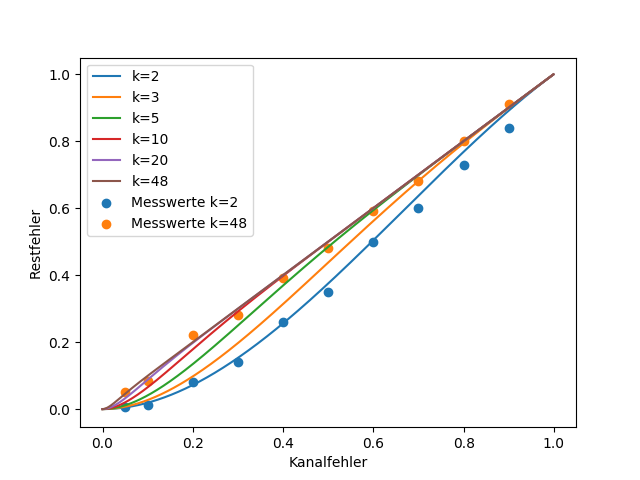
\includegraphics[scale=0.7]{plots}
    \end{center}

    \noindent
    Die Werte wurden mit folgender Formel berechnet:

    Sei \(k\) die Gruppengröße:
    \begin{equation}
        \begin{aligned}
            P_{Rest}
            & = \frac{ \sum_{i=2}^{n =k+1} \binom{n}{i} \cdot P^k \cdot (1-P)^{n-i} \cdot \frac{i \cdot k}{n}}
            {k} \\
            & = \sum_{i=2}^{n =k+1} \binom{n}{i} \cdot P^k \cdot (1-P)^{n-i} \cdot \frac{i}{n}\\
        \end{aligned}
    \end{equation}

    \noindent
    Zum Plotting habe ich Pyhton benutzt.

    \begin{lstlisting} [language=Python]
    def g(P, k):
        n = k + 1
        sum = 0
        for i in range(2, n + 1):
            sum += scipy.special.comb(n, i) * P ** i \
            * (1 - P) ** (n - i) * (i / float(n))
        return sum

    [...]

    k_list = [2, 3, 5, 10, 20, 48]
    for k in k_list:
        x = np.arange(0.0, 1.0, 0.001)
        y = g(x, k)
        plt.plot(x, y, label='k=' + str(k))
    \end{lstlisting}

    \noindent
    Die gemessenen Werte korrelieren sehr gut mit den berechneten, deswegen erübrigt sich die Diskussion.

    \section{Kompatibilität}
    Der Client und Server sind mit VLC nicht kompatibel.


    \section{Vorschläge}

    In Aufgabe 4 war gefordert, die Paketverluste und eine Variable Verzögerung im Netz zu simulieren.
    Ich dachte zuerst, wir sollen eine Verzögerung einbauen, zum Beispiel:

    \begin{lstlisting}[language=Java]
        Thread.sleep(100);
    \end{lstlisting}

    \noindent
    Anscheinend war aber die Aufgabe, die Verzögerung \textbf{durch} die Unterdrückung von Paketen zu realisieren.
    Mein Vorschlag wäre, die Aufgabe anders zu formulieren.
\end{document}